% !TeX encoding = UTF-8
% !TeX spellcheck = en_US

\documentclass[compress,ignorenonframetext,aspectratio=1610,handout]{beamer}
\usepackage[USenglish]{babel}
\usepackage[utf8]{inputenc}
\usetheme{Cantabria}
\usepackage{url}
\usepackage{xfrac}
\usepackage{amsmath}
\usepackage{latexsym}
\usepackage{amssymb}
\usepackage{mathtools}
\usepackage[ruled]{algorithm2e}
\usepackage{graphicx}
\usepackage{alphabeta}
\usepackage{textcomp}


\usepackage[ruled]{algorithm2e}
\usepackage{subfig}
\usepackage{multirow}
\usepackage{booktabs}
\usepackage{xcolor}
\usepackage{svg}

\usepackage{calc}  
\usepackage{enumitem}  
\usepackage[compatibility=false]{caption}
\usepackage{textcomp}
\usepackage{ulem}
\usepackage{listings}
\usepackage{multimedia}
\usepackage{subfig}
\usepackage{svg}
\usepackage[export]{adjustbox}

\setbeamerfont{footnote}{size=\tiny}

\DeclareMathOperator*{\argmax}{arg\,max}
\DeclareMathOperator*{\argmin}{arg\,min}

\newcommand\blfootnote[1]{%
  \begingroup
  \renewcommand\thefootnote{}\footnote{\tiny{#1}}%
  \addtocounter{footnote}{-1}%
  \endgroup
}

% \captionsetup{compatibility=false}


\def\xrow{
	\begin{bmatrix}
    x_1 & x_2 & \cdots & x_m
\end{bmatrix}}

\def\xsrow{
	\begin{bmatrix}
    \mathbf{X}_{:,1} & \mathbf{X}_{:,2} & \cdots & \mathbf{X}_{:,m}
\end{bmatrix}}

\def\xcol{
\begin{bmatrix}
    x_1 \\
    x_2 \\
    \vdots \\
    x_m
\end{bmatrix}}

\def\xscol{
\begin{bmatrix}
    \mathbf{X}_1 \\
    \mathbf{X}_2 \\
    \vdots \\
    \mathbf{X}_m
\end{bmatrix}}

\def\xmat{
	\begin{bmatrix}
		X_{1,1} & X_{1,2} & \cdots & X_{1,n} \\
		X_{2,1} & X_{2,2} & \cdots & X_{2,n} \\
		\vdots  & \vdots  & \ddots & \vdots  \\
		X_{m,1} & X_{m,2} & \cdots & X_{m,n} 
	\end{bmatrix}
}

\newcommand\norm[1]{\left\lVert#1\right\rVert}

 
\definecolor{codegreen}{rgb}{0,0.6,0}
\definecolor{codegray}{rgb}{0.5,0.5,0.5}
\definecolor{codepurple}{rgb}{0.58,0,0.82}
\definecolor{backcolour}{rgb}{0.95,0.95,0.92}

\lstdefinestyle{mypy}{
    backgroundcolor=\color{backcolour},   
    commentstyle=\color{codegreen},
    keywordstyle=\color{magenta},
    numberstyle=\tiny\color{codegray},
    stringstyle=\color{codepurple},
    basicstyle=\footnotesize\ttfamily,
    breakatwhitespace=false,         
    breaklines=true,                 
    captionpos=b,                    
    keepspaces=true,                 
    numbers=left,                    
    numbersep=5pt,                  
    showspaces=false,                
    showstringspaces=false,
    showtabs=false,                  
    tabsize=2
}

\captionsetup[figure]{labelformat=empty}% redefines the caption setup of the figures environment in the beamer class.


\usepackage[minnames=1,maxnames=1,style=authoryear,backend=bibtex]{biblatex}
\addbibresource{bibliography.bib}

\usepackage{pdfpages}

%\newcommand{\textapprox}{\hbox{$\null\approx\,\null$}}
\newcommand{\textthen}{\hbox{$\null\Rightarrow\,\null$}}


\newcommand{\sign}{\operatornamewithlimits{sign}}
\DeclareMathOperator{\mean}{mean}
\def\RR{\mathbb{R}}
\def\ZZ{\mathbb{Z}}
\def\NN{\mathbb{N}}
\DeclareMathOperator{\vect}{vec}
\DeclareMathOperator{\rtwo}{R}

\usepackage{tikz}
\usetikzlibrary{decorations.pathreplacing}
\newcommand\tikzmark[1]{
  \tikz[remember picture,overlay] \coordinate (#1);
}


\newcommand{\smiley}{\tikz[baseline=-0.75ex,black]{
		\draw circle (2mm);
		\node[fill,circle,inner sep=0.5pt] (left eye) at (135:0.8mm) {};
		\node[fill,circle,inner sep=0.5pt] (right eye) at (45:0.8mm) {};
		\draw (-145:0.9mm) arc (-120:-60:1.5mm);
	}
}

\newcommand{\frownie}{\tikz[baseline=-0.75ex,black]{
		\draw circle (2mm);
		\node[fill,circle,inner sep=0.5pt] (left eye) at (135:0.8mm) {};
		\node[fill,circle,inner sep=0.5pt] (right eye) at (45:0.8mm) {};
		\draw (-145:0.9mm) arc (120:60:1.5mm);
	}
}

\newcommand{\neutranie}{\tikz[baseline=-0.75ex,black]{
		\draw circle (2mm);
		\node[fill,circle,inner sep=0.5pt] (left eye) at (135:0.8mm) {};
		\node[fill,circle,inner sep=0.5pt] (right eye) at (45:0.8mm) {};
		\draw (-135:0.9mm) -- (-45:0.9mm);
	}
}

\newcommand{\tabitem}{%
  \usebeamertemplate{itemize item}\hspace*{\labelsep}}

\usepackage{mdwlist}
\usepackage{lmodern}

\addtobeamertemplate{theorem begin}{\normalfont}{}

\usefonttheme[onlymath]{serif}


% \useinnertheme{circles}
% \newenvironment{trienv}{\only{\setbeamertemplate{items}[triangle]}}{}
% \newenvironment{squareenv}{\only{\setbeamertemplate{items}[square]}}{}

%\defbeamertemplate{itemize item}{circle}{\small\raise0.5pt\hbox{\textbullet}}

% \usepackage{mathptmx}
% \usepackage[scaled=0.9]{helvet}
% \usepackage{courier}

\title[Drug repurposing for COVID-19 with Real World Evidence]{Drug repurposing for COVID-19 using explainable machine learning and mechanistic models of signal transduction circuits related to SARS-CoV-2 infection with real world data validation}
\author{Carlos Loucera}
\institute{
	Bioinformatics Area, Andalusian Public Foundation Progress and Health-FPS, 41013 Sevilla, Spain \\
	Institute of Biomedicine of Seville, IBiS, University Hospital Virgen del Rocío/CSIC/University of Seville, 41013 Sevilla, Spain
}
\date{
	MAQC 2022 \\ 
	2022 September 26}

\begin{document}

% standard title page2
%\frame[plain]{\titlepage}
%\setbeamertemplate{footline}{}

% title page with custom logos
\begin{frame}[plain]
	\vspace{\stretch{1}} % push title down a little
	\titlepage % write standard title page
	\vspace{\stretch{.5}}
	% vertically center logos with raisebox

	\hspace{\stretch{1}}
	\raisebox{-0.5\height}{
\includegraphics[width=8.0cm]{figs/logos/fps_logo}}
	\hspace{\stretch{1}}
	\raisebox{-0.5\height}{
\includegraphics[width=3.5cm]{figs/logos/ibi_logo.png}}
	\hspace{\stretch{1}}
	\raisebox{-0.5\height}{
\includegraphics[width=1.5cm]{figs/logos/logo-vectorizado}}
	\hspace{\stretch{1}}
	% \raisebox{-0.5\height}{\includegraphics[width=1.5cm]{figs/US-marca-digital-cuadrada.eps}}
	\addtocounter{framenumber}{-1} 
\end{frame}

%%%%%%%%%%%%%%%%%%%%%%%%%%%%%%%%%%%%%%%%%%%%%%%
\section{Introduction}


\begin{frame}{Knowledge paradigm}
	\begin{columns}
		\column{0.99\textwidth}
		\begin{figure}
			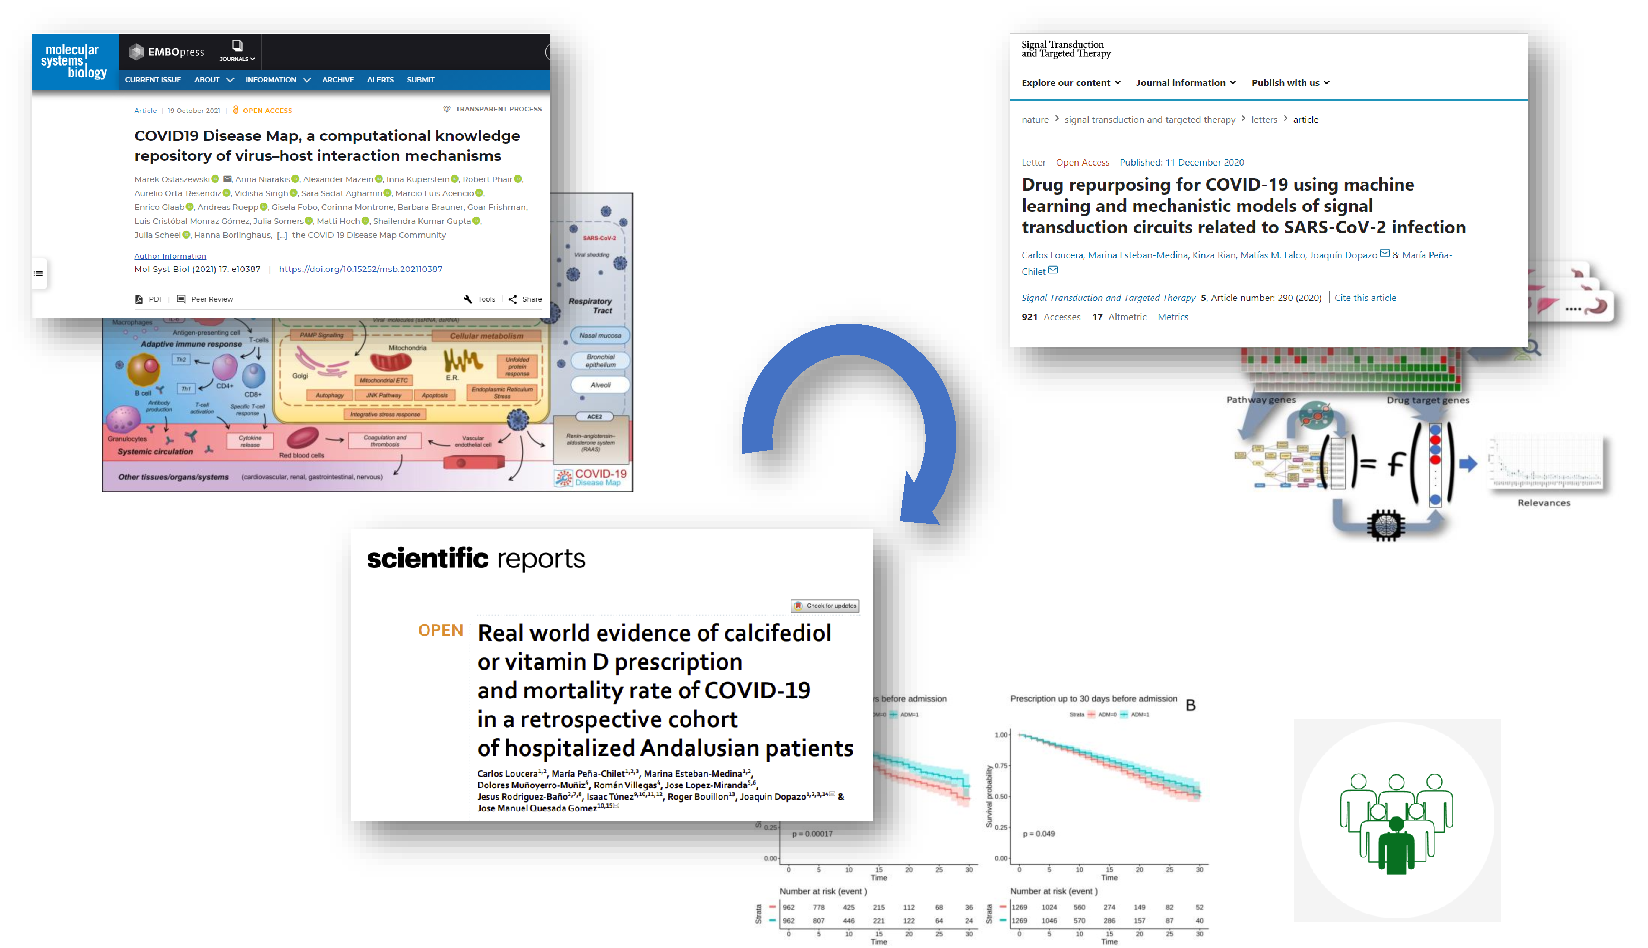
\includegraphics[width=0.85\textwidth]{figs/methods/knowdge_paradigm-crop.pdf}
		\end{figure}

	\end{columns}
\end{frame}



\begin{frame}{Knowledge discovery}

	\textbf{Living Contradiction} is a fascinating, honest examination of that genuine contradiction faced 
	by teachers in reconciling the effort made to \emph{encourage} young people towards \emph{independent 
	critical thinking}, with the simultaneous sense of \emph{responsibility to instruct} and insist 
	on a particular behavior. \\

	\vspace*{1em}

	\textbf{Trustworthiness} \\

	\vspace*{1em}

	The \textbf{WHY} is as important as the \textbf{WHAT} \\

	\blfootnote{\url{https://www.crownhouse.co.uk/product-review/10842}}

\end{frame}

\section{Methods}


\begin{frame}{Building a COVID-19 Disease Map}
	\begin{columns}
		\begin{column}{0.6\textwidth}
			\centering
			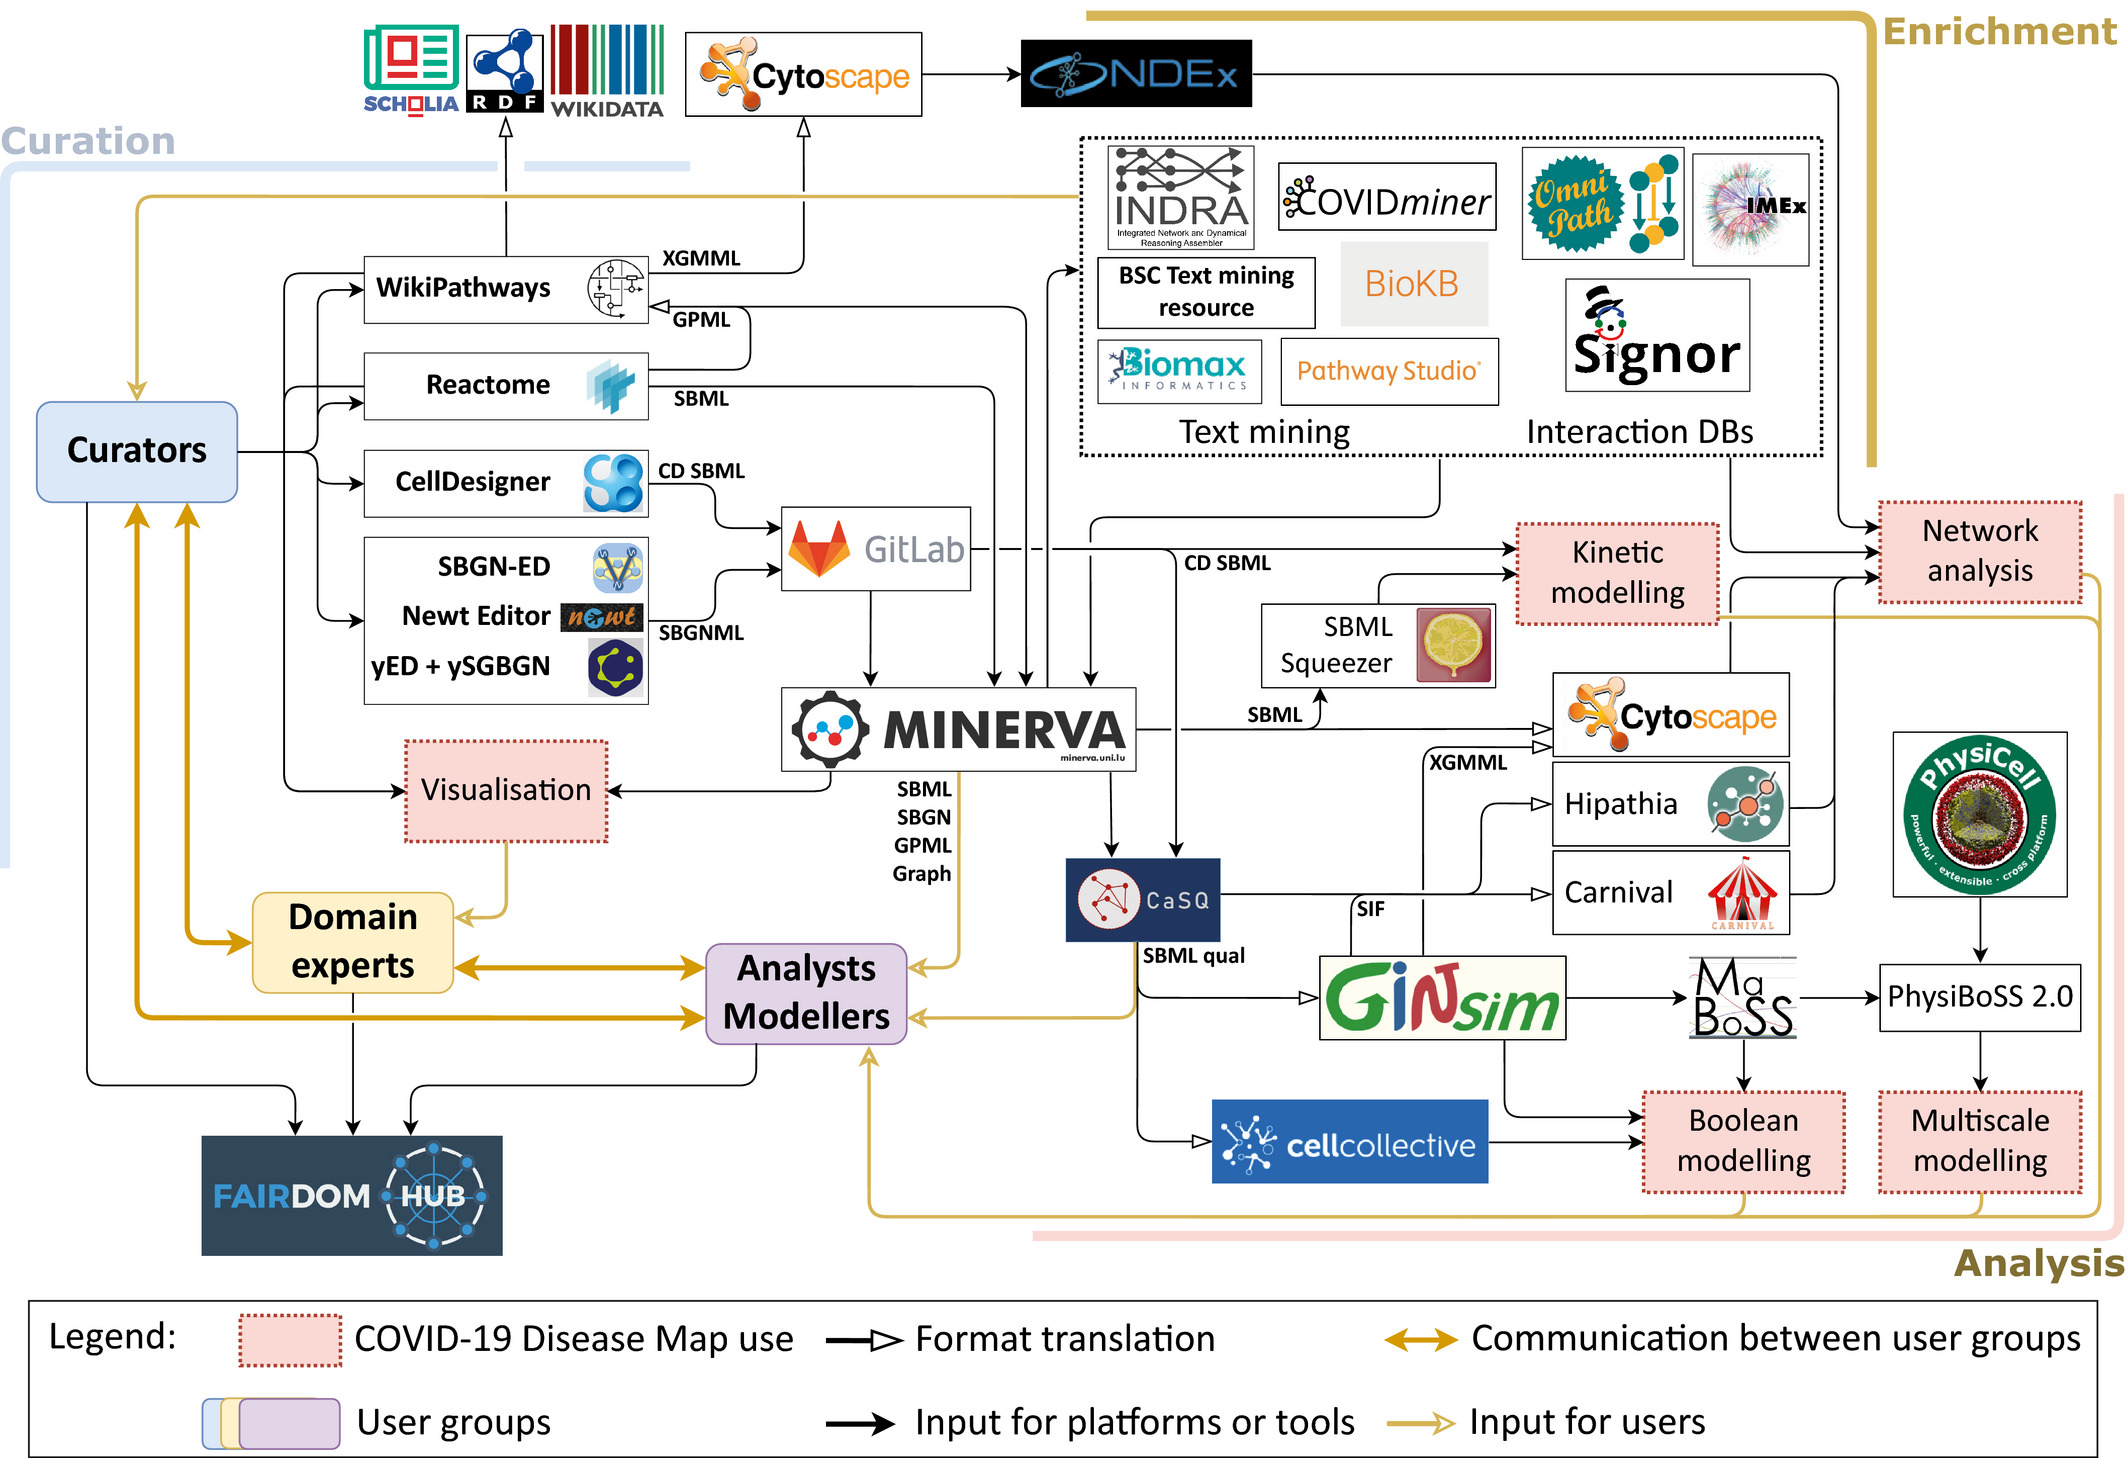
\includegraphics[width=0.9\textwidth]{figs/methods/covid19-diseasemap-consrtium.jpg}
			\captionof{figure}{COVID-19 Disease Map\footnotemark }

		\end{column}

		\pause

		\begin{column}{0.4\textwidth}

		\end{column}

	\end{columns}
	\footnotetext[1]{\fullcite{ostaszewski2021covid19}}

\end{frame}

\begin{frame}{Building a COVID-19 Disease Map}
	\begin{columns}
		\begin{column}{0.6\textwidth}
			\centering
			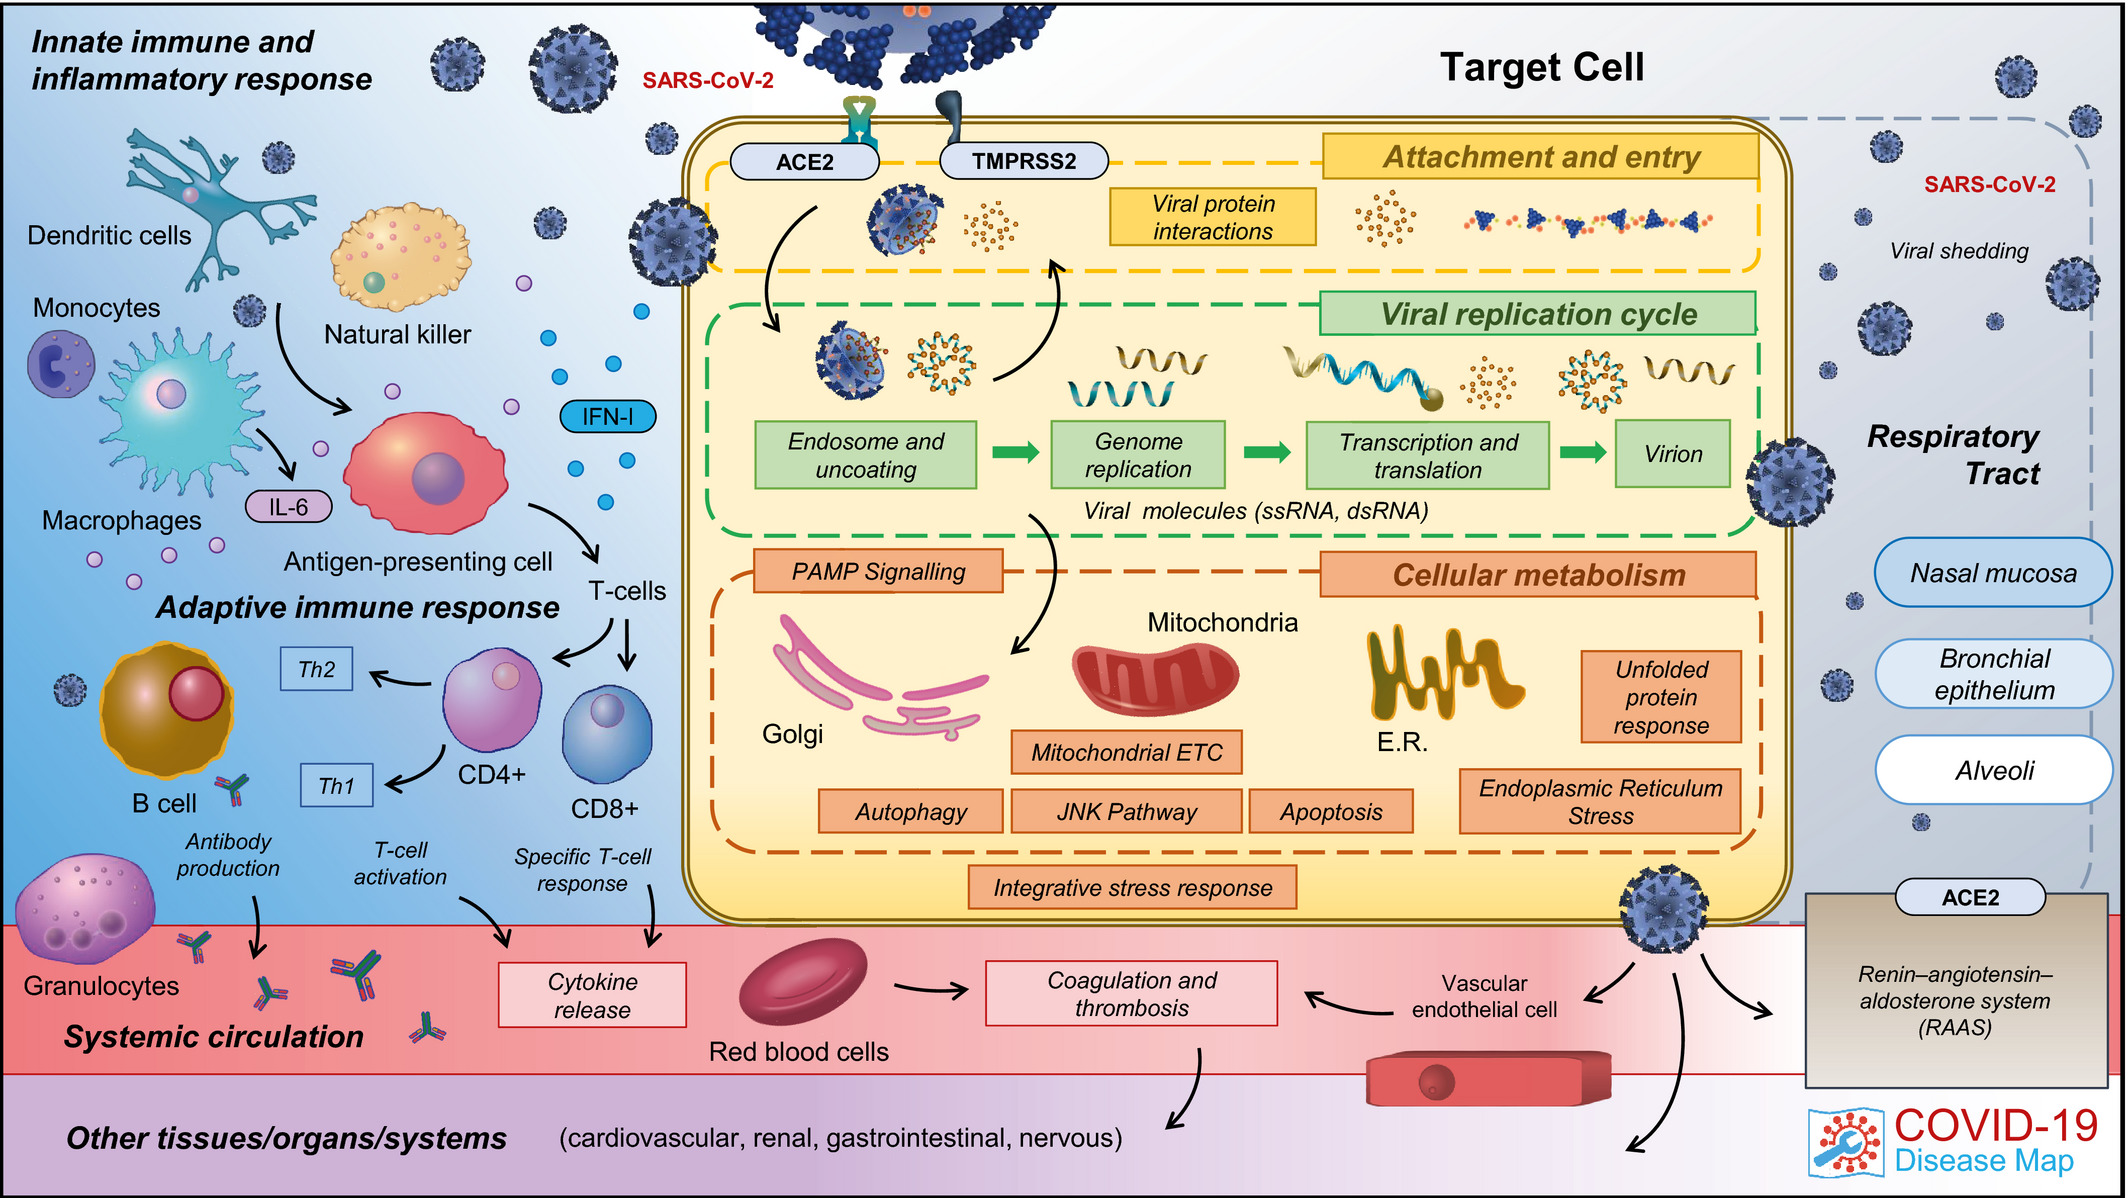
\includegraphics[width=0.9\textwidth]{figs/methods/covid19_diseasemap.jpg}
			\captionof{figure}{COVID-19 Disease Map\footnotemark }

		\end{column}

		\pause

		\begin{column}{0.4\textwidth}
			\centering
			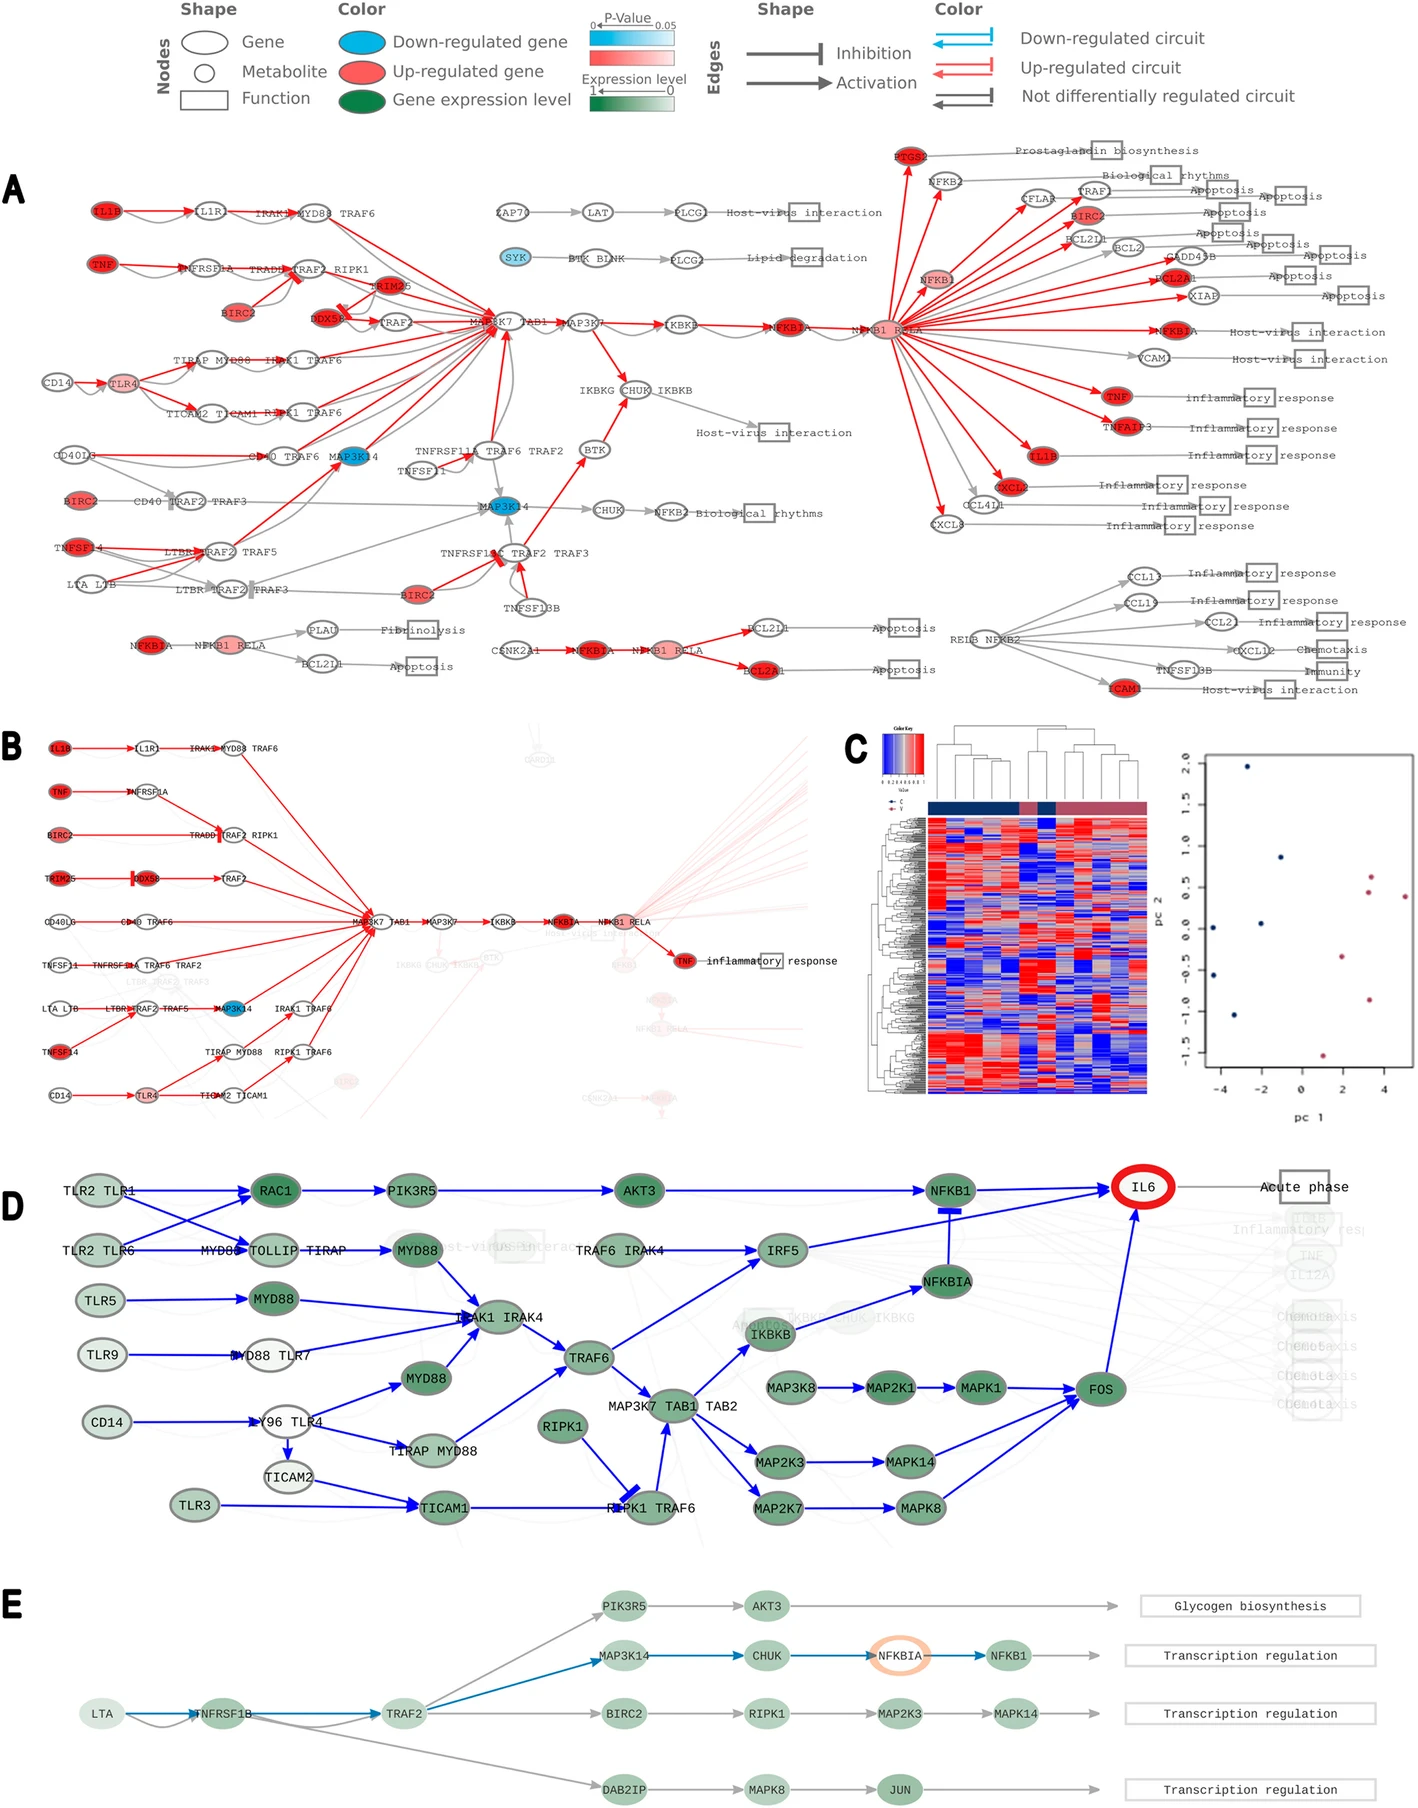
\includegraphics[width=0.8\textwidth]{figs/methods/covipathia.png}
			\captionof{figure}{(Simplified) COVID-19 Disease Map\footnotemark }

		\end{column}

	\end{columns}
	\footnotetext[1]{\fullcite{ostaszewski2021covid19}}
	\footnotetext[2]{\fullcite{rian2021mechanistic}}
\end{frame}



\begin{frame}{Drug repurposing schema}
	\begin{columns}
		\column{0.99\textwidth}
		\begin{figure}
			
\includegraphics[width=0.99\textwidth]{figs/methods/COVI-19_drugRepo.png}
		\end{figure}

	\end{columns}
\end{frame}


\section{Results}


\begin{frame}{Covariate-Adjusted LHR by Treatment}
	\begin{columns}
		\column{0.99\textwidth}
		\begin{figure}
			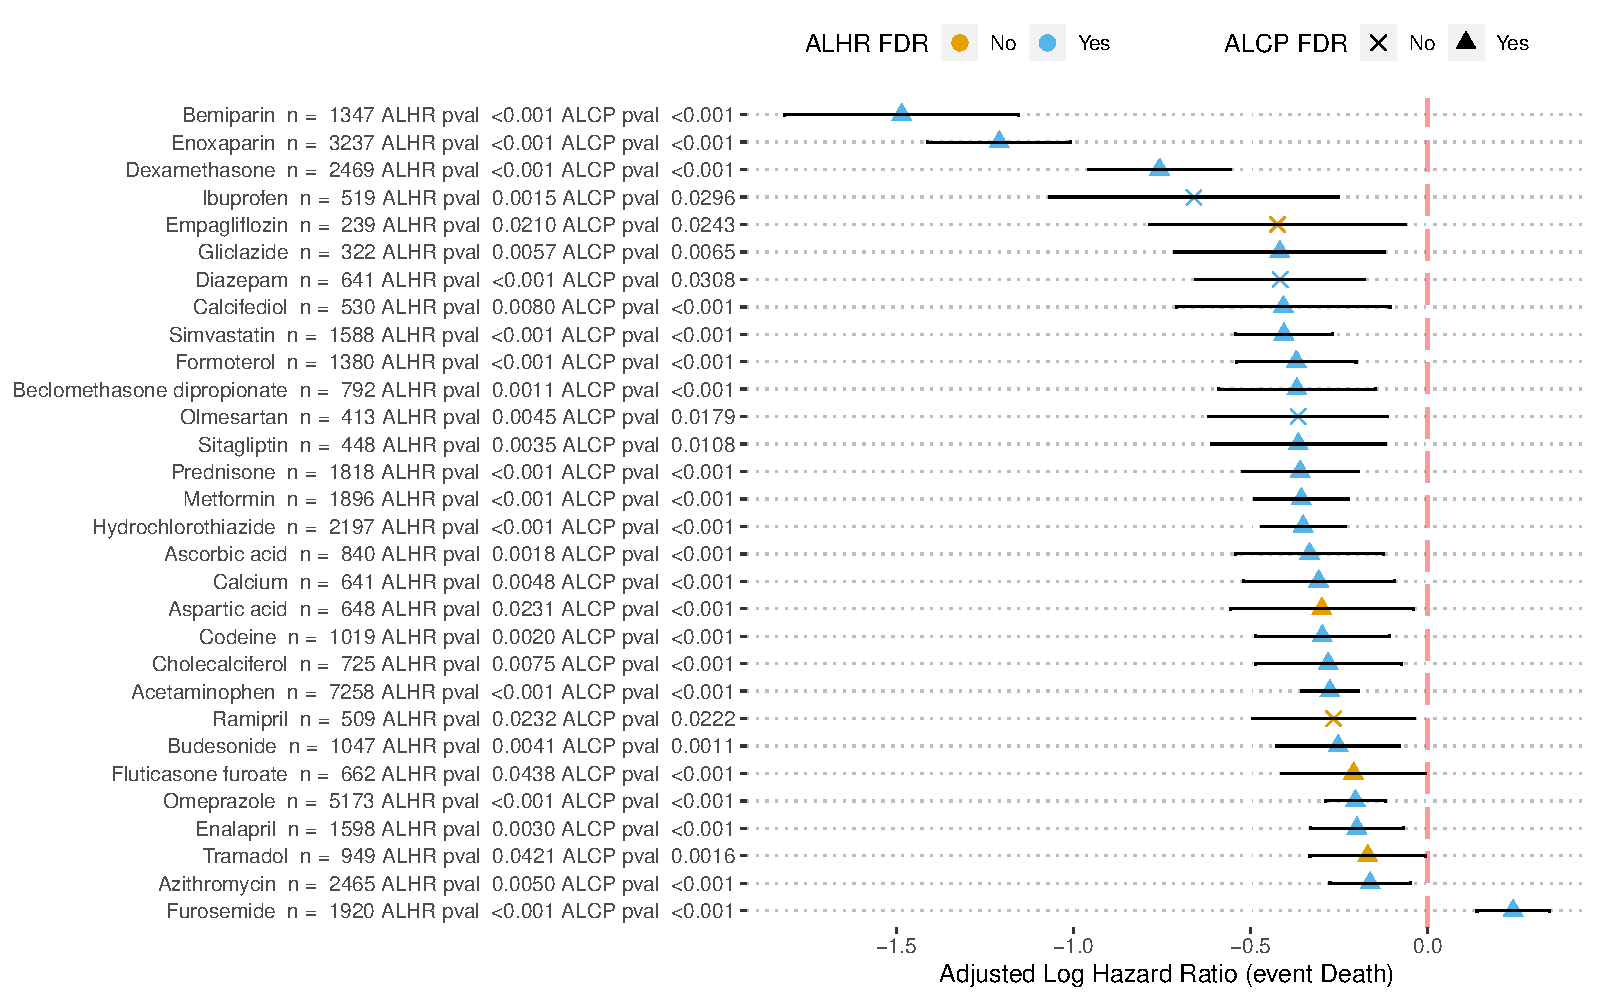
\includegraphics[width=0.88\textwidth]{figs/results/bps_covid_repurposing_summary.pdf}
		\end{figure}

	\end{columns}
\end{frame}

\begin{frame}{Covariate-Adjusted Lymphocyte trend}
	\begin{columns}
		\column{0.5\textwidth}
		\begin{figure}
			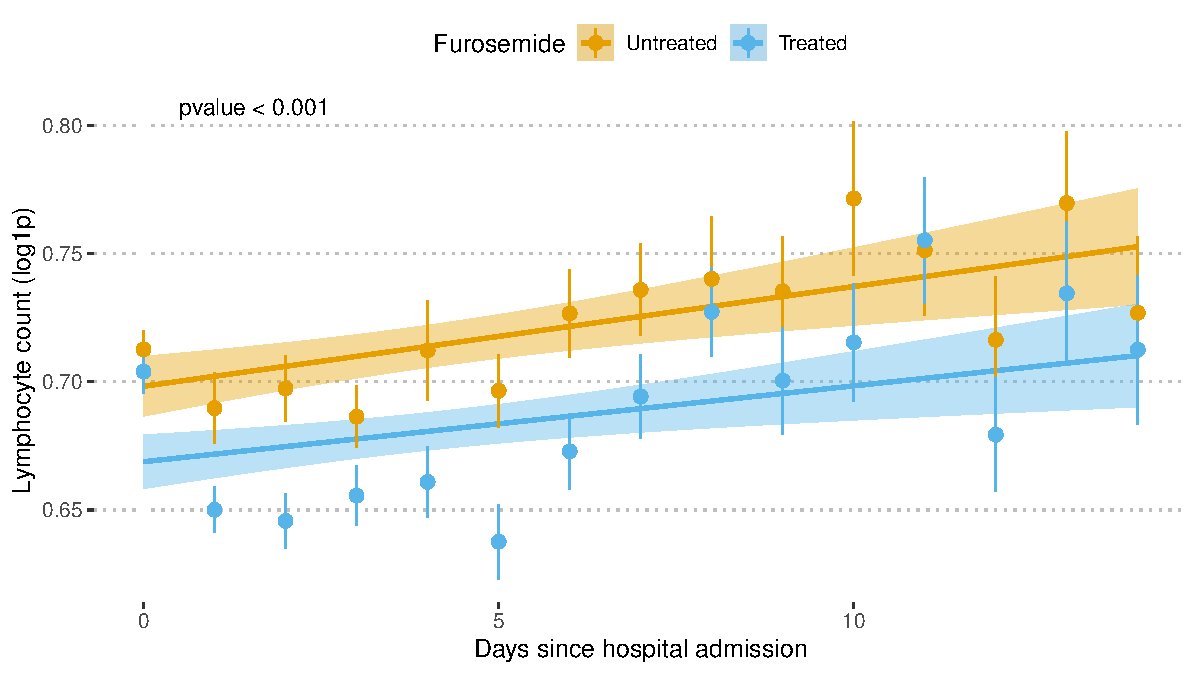
\includegraphics[width=0.8\textwidth]{figs/results/db00695_furosemide_lymphocite_progression.pdf}	
		\end{figure}

		\column{0.5\textwidth}
		\begin{figure}
			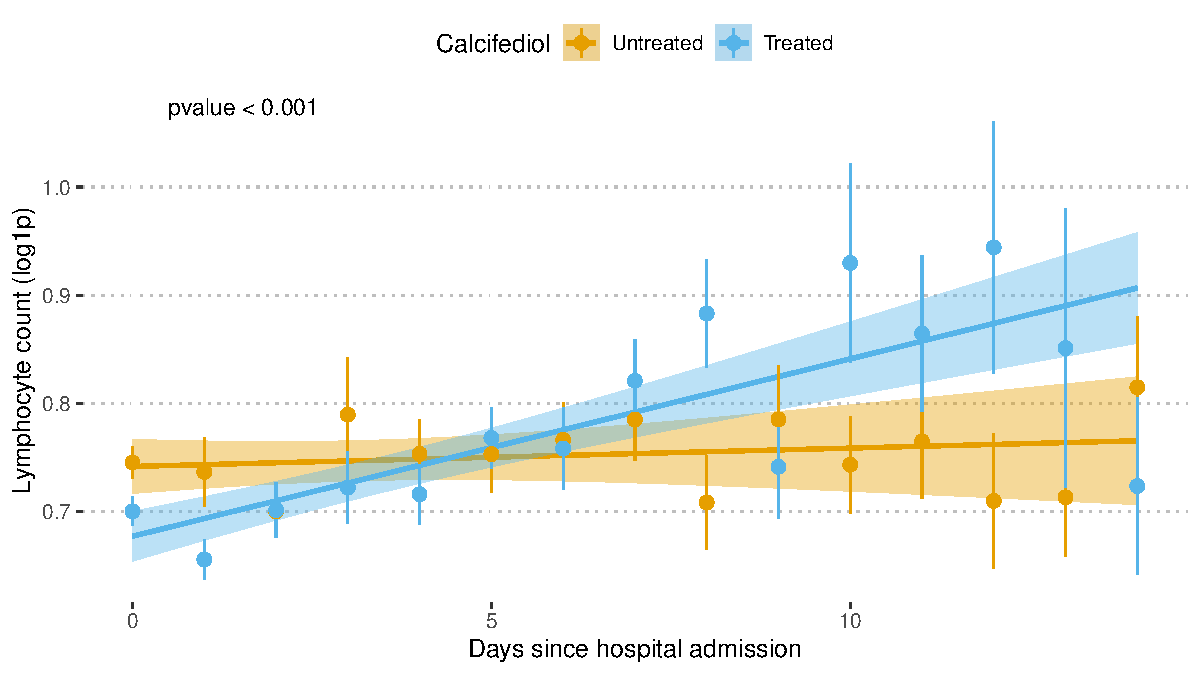
\includegraphics[width=0.8\textwidth]{figs/results/db00146_calcifediol_lymphocite_progression.pdf}	
		\end{figure}

	\end{columns}

	\begin{figure}
		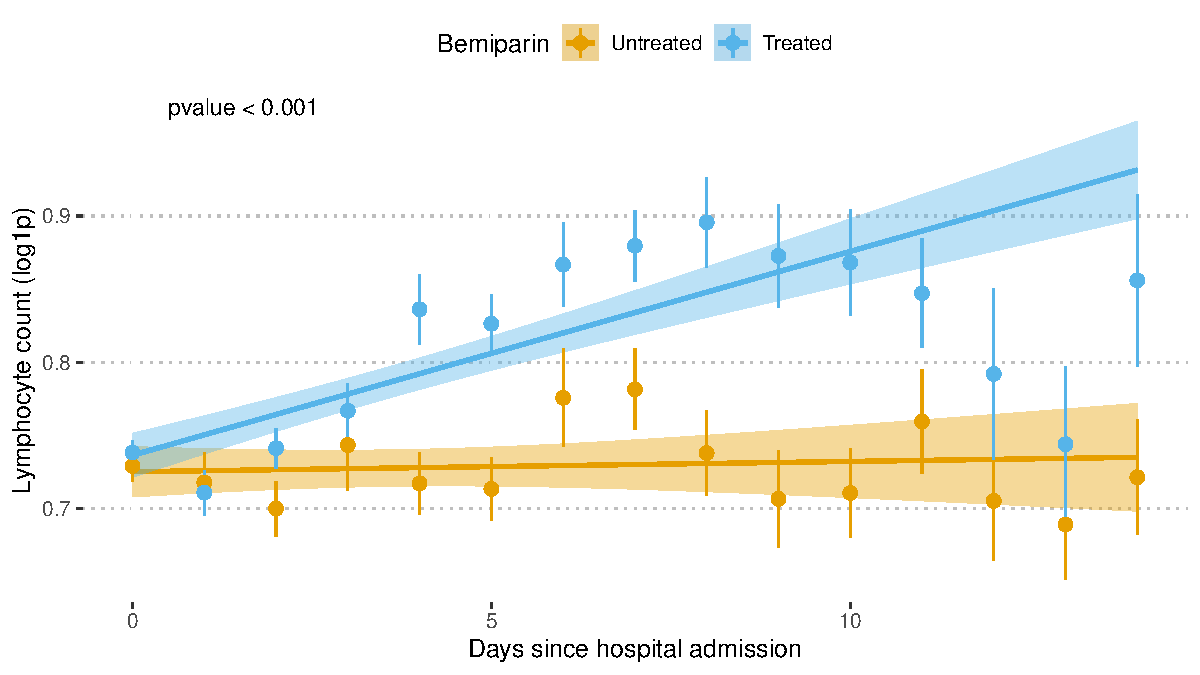
\includegraphics[width=0.4\textwidth]{figs/results/db09258_bemiparin_lymphocite_progression.pdf}	
	\end{figure}


\end{frame}


\section{Thanks}

	% \begin{frame}{The future}

	% 	\begin{columns}

	% 		\column{0.5\textwidth}
	% 		\centering\includegraphics[width=0.6\textwidth]{figs/mse_oracle.jpg}

	% 		\column{0.5\textwidth}

	% 		\centering\includegraphics[width=0.8\textwidth]{figs/xkcd_machine_learning.png}
			
	% 	\end{columns}

	% 	\blfootnote{\url{https://www.flickr.com/photos/69969104@N00/3351804379/}}
	% 	\blfootnote{\url{https://xkcd.com/1838/}}
	% \end{frame}



	\begin{frame}{}
		\begin{center}
			{\fontsize{40}{50}\selectfont Thank You!}
		\end{center}
	\end{frame}


	\begin{frame}{Personal funding. Contact: \url{carlos.loucera@juntadeandalucia.es}}

		\raisebox{-0.45\height}{
\includegraphics[width=5cm]{figs/logos/logo_postdoc_consejeria.jpeg.jpg}}
		\hspace{\stretch{1}}
		\raisebox{-0.45\height}{
\includegraphics[width=3cm]{figs/logos/logo_postdoc_eu.png}}
		\hspace{\stretch{1}}

		\vspace{0.3cm}

		Carlos Loucera postdoctoral contract \texttt{PAIDI2020-DOC\_00350} is funded by Junta de Andalucía and co-funded by the European Social Fund (FSE) 2014-2020

		\vspace{0.3cm}

		\begin{center}
			\raisebox{-0.5\height}{
\includegraphics[width=3cm]{figs/logos/logo_postdoc_jdaeu.png}}
		\end{center}
	\end{frame}

	\begin{frame}
		\vspace*{-1pt}
		\makebox[\linewidth]{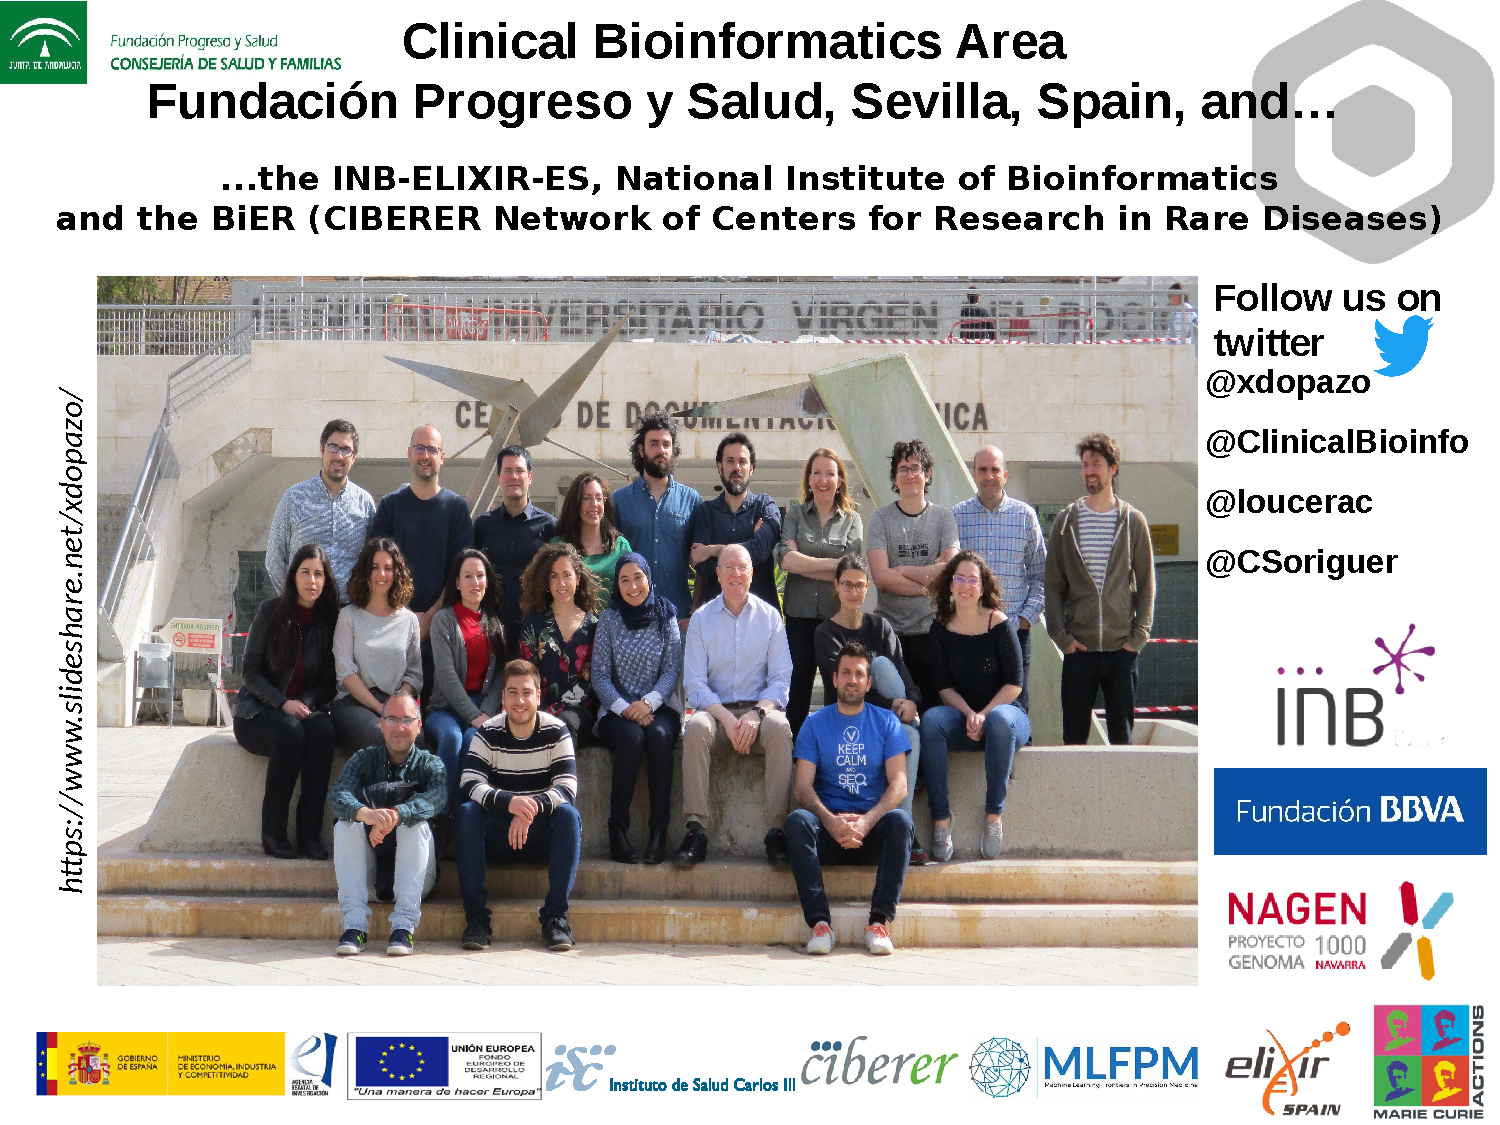
\includegraphics[page=1,width=0.65\paperwidth]{figs/people/fps_final_slide.pdf}}
	\end{frame}

\end{document}
